\documentclass[conference]{IEEEtran} \IEEEoverridecommandlockouts \usepackage{graphicx}

\def\code#1{\texttt{#1}}

\usepackage{listings}
\usepackage{color}

\definecolor{dkgreen}{rgb}{0,0.6,0}
\definecolor{gray}{rgb}{0.5,0.5,0.5}
\definecolor{mauve}{rgb}{0.58,0,0.82}

\lstset{frame=tb, language=C++, aboveskip=3mm, belowskip=3mm, showstringspaces=false,
  columns=flexible, basicstyle={\small\ttfamily}, numbers=none,
  numberstyle=\tiny\color{gray}, keywordstyle=\color{blue}, commentstyle=\color{dkgreen},
  stringstyle=\color{mauve}, breaklines=true, breakatwhitespace=true, tabsize=3}

%opening
\title{Micro-benchmarking of C++ containers} \author{Victor BERNARD, Samuel JUNG, François
  PANSERA}

\begin{document}

\maketitle
	
\begin{abstract}
	
This paper presents a C++ library for benchmarking STL containers. It allows users to
determine, for a given algorithm, which container is the fastest based on the size of the
dataset. Its architecture enables C++ developers to easily configure and quickly adapt the
software to their specific problem. This software has been specifically designed for cases
where the dataset is small, making it challenging for developers to determine the optimal
choice of container without empirical testing. We then verified the effectiveness of the
software on the problem of choosing between \code{std::vector} and
\code{std::unordered\_set}.

\end{abstract}

\section{Introduction}

Maximizing the performance of a modern C++ program is a challenge. There are several
abstraction libraries available to simplify programming, such as STL or Boost. While these
abstractions are optimized, performance can vary depending on their usage, making
performance prediction particularly difficult.

Some tools exist to address this problem, such as Warrior1
\cite{arXiv:2010.09583}. Warrior1 is a tool that identifies optimization issues in a
program that would be difficult to spot using conventional debugging and optimization
tools. It detects problems such as short-lifetime instances or passing objects by value
instead of by reference. However, Warrior1 does not provide information on whether a
different type of container would be more efficient than the one being used.

The STL and Boost libraries add many containers that simplify the work of developers, such
as vectors, lists, or unordered sets. Each type of container is developed by optimizing a
specific aspect of its use. The \code{std::vector} \cite{stllibrary} is a dynamic array
with fast access to data. The \code{std::list} \cite{stllibrary} is a dynamic array that
allows for quick addition and removal of data. The \code{std::unordered\_set}
\cite{stllibrary} is an associative container that stores unique elements without a
particular order. The Boost library also has an implementation of this last container
\code{boost::unordered\_set} \cite{boostlibrary}, adding some feature to the original
container.

However, it is difficult to determine which container will be the most optimized for a
specific use case with a specific data structure and size, whether it is in terms of
execution time or memory usage. The work of Vreda Pieterse, Derrick G. Kourie, Bruce
W. Watson, and Loek Cleophas \cite{https://doi.org/10.1145/1899503.1899530} precisely
compares the performance (time and memory) of different bit containers for a 1000 x 1000
array using a benchmark algorithm and shows significant performance differences.

Even in cases of simple data with conventional instructions, it can be difficult to
determine which container is the best based on the size of the data and the execution
environment. Often, when a container is optimized for a specific task, the difference is
most noticeable for large data sets, and sometimes it may even be less efficient for small
data sets compared to other more traditional containers. This phenomenon is evident in the
previously mentioned article\cite{https://doi.org/10.1145/1899503.1899530}; in terms of
execution time, \code{std::vector<char>} outperforms \code{boost::dyn\_bitset} or
bm::bvector for small data sets, but the opposite is true for larger data sets. The same
phenomenon likely exists between \code{std::unordered\_set} and \code{std::vector} when it
comes to determining whether the container contains a particular element or
not. \code{std::unordered\_set} uses hashing for such operations and should be more
efficient, but when the size of the data set is small enough, \code{std::vector} could be
faster.

In the realm of small data sets, there is potentially a threshold beyond which one
container is faster than another. Such a threshold will depend on the containers, the
algorithm, and the execution environment. The purpose of this article is to propose a
benchmark program that allows easy testing of cases as stated earlier and finding data
size thresholds if they exist. This will enable developers to choose the appropriate
container for small data sets and optimize their programs to the fullest extent.

\section{Implementation}

This section will explain how our benchmarking program was designed to
produce reliable results and provide flexibility in benchmarking
different algorithms.

\subsection{Protocol}

Since we are interested in the performance of containers on small datasets, the metric we
are concerned with is the execution time. However, the memory space used will be
disregarded. The idea is to measure the execution time of a specific algorithm for each
type of container. It is essential that our program provides reliable and meaningful
results. To achieve this, we measure only the execution of the algorithm using the chrono
library and its \code{chrono::high\_resolution\_clock}. This library allows us to measure
time with nanosecond precision. Considering that the program may be executed in highly
multithreaded environments such as a Windows 10 or Ubuntu computer, and since the
measurement is in nanoseconds, there is a risk that the measurement may be impacted by its
execution environment. To minimize this risk, it is important to run the program with a
high priority and have few concurrent processes running on the computer. Another
measure we have taken into account to ensure the reliability and significance of the
measurements is the ability to repeat each measurement as many times as desired. It is
possible, for example, to repeat each measurement 10 times and remove the 2 measurements
that deviate the most from the median. This should help us reduce the noise in our
measurements caused by the environment. Note that the number of measurements and how they
are treated remains the user's choice.

Next, we need to take measurements for each type of container for multiple data set
sizes. Since the goal is to find the threshold data size at which the fastest container
changes, we want to plot a graph of execution time against the data set. Considering that
we are interested in small data sets, we can vary our data set size from 0 to 1000
elements. The variation of the data set can be linear (with a step of 10 to 50 elements)
since the magnitude of the data set doesn't vary much.

\subsection{Architecture}

Our benchmarking software needs to be able to measure the performance of containers for
multiple algorithms. The software architecture is crucial to enable the modification of
benchmark and algorithm parameters. The goal is to allow for easy and quick modification
of these aspects. If another user wants to know which container to use for their specific
case, they should be able to do so without having to understand the entire functioning of
the benchmarking software.

That's why we have implemented the following architecture, mainly consisting of 4 classes:

\begin{figure}[!h]
	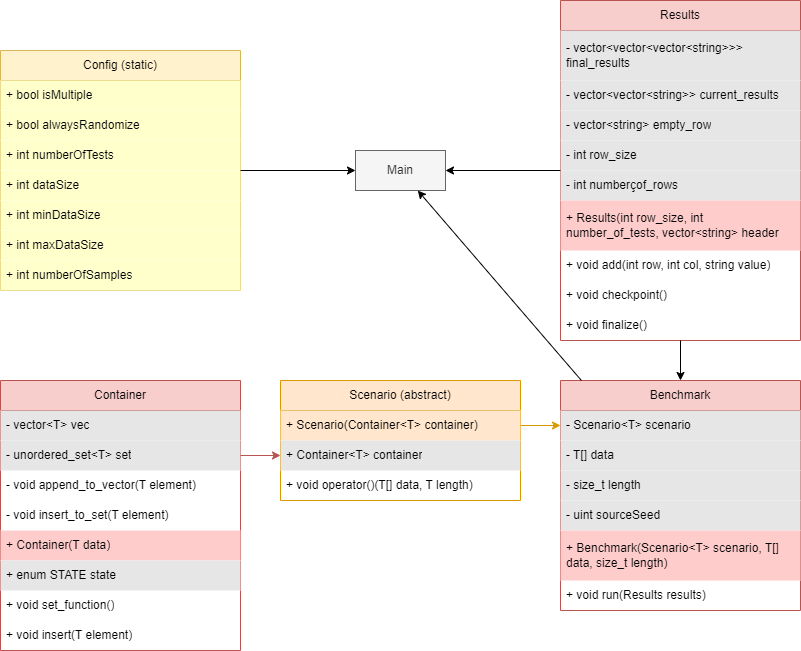
\includegraphics[width=9cm]{Diagram/architecture.png}
	\caption{Class diagram}
	\label{class diagram}
\end{figure}

\begin{itemize}
	\item Container \ref{class diagram}: This class contains an instance of each type
          of container being tested and serves as an abstraction for using the operations
          of these containers. It uses an enumerator \code{STATE} to define which
          container is being used at any given moment.
	\item Scenario \ref{class diagram}: This abstract class utilizes the container and
          contains the benchmarked algorithm.
	\item Benchmark \ref{class diagram}: This class utilizes the scenario, executes
          its algorithm as many times as necessary, measures its performance, and sends
          the results.
	\item Results \ref{class diagram}: This class is called by the benchmark object
          and store all result data to create the final CSV file.
	\item Config \ref{class diagram}: This static class contains various execution
          parameters for the benchmark, such as the size of the dataset, the number of
          repeated measurements, etc.
\end{itemize}

\subsection{How to use}

In order to employ the benchmark library, users are initially required to configure the
benchmarking process by modifying the \code{config.hpp} file. Subsequently, they need to
include and create a functor that inherits from the Scenario class. Within the
\code{operator()} method of this functor, the benchmarking procedure must be implemented,
and any operations involving containers should be executed using the methods of the
container property. To conduct the benchmarking process, users need to supply an instance
of this functor to a benchmark and invoke the \code{run} method. These steps encompass the
essential user requirements. Furthermore, we offer illustrative benchmarking procedures
along with their corresponding outcomes as examples.

Here is an example of a benchmark procedure implementation
\begin{lstlisting}
	struct Test : Scenario<int> { Test(Container<int> *container) :
          Scenario<int>(container) {}
		
		void operator()(int data[], int length) override { for (int i = 0; i <
                  length; i++) { container->insert(data[i]); } } };
\end{lstlisting}

In order to cover a variety of use cases, we decided to implement a configuration file
named \code{config.hpp}. We therefore have 2 types of test defined by the
\code{isMultiple} variable:
\begin{itemize}
	\item Single tests, testing a single data size (\code{false}).
	\item Multiple tests, a set of single tests (\code{true}).
\end{itemize}

For each test we have the following parameters:
\begin{itemize}
	\item Whether to generate random data for each test, or for each data size
          (\code{alwaysRandomize}).
	\item The number of tests to be run for each data size (\code{numberOfTests}).
\end{itemize}

In the case of a single test, we have the size of the data to be tested (\code{dataSize}).

In the case of a multiple test, we have the following parameters:
\begin{itemize}
	\item Minimum data size (\code{minDataSize}).
	\item Maximum data size (\code{maxDataSize}).
	\item Number of samples: the higher this value, the more data sizes will be tested
          (\code{numberOfSamples}).
\end{itemize}

Here are the complete contents of the configuration file:
\begin{lstlisting}
	#ifndef CONFIG define CONFIG
	
	struct Config { // Should we execute tests for multiple sizes?  static const bool
          isMultiple = true;
		
		// [PER TEST] // Should we randomize the data once, or for every
                execution?  static const bool alwaysRandomize = true; // For each size,
                how much tests should be executed ?  static const int numberOfTests = 50;
		
		// [FOR A SINGLE TEST] only if isMultiple=false // The size of the
                randomized data for that test static const int dataSize = 50;
		
		// [FOR MULTIPLE TESTS] only if isMultiple=true // The minimum size of the
                randomized data static const int minDataSize = 1; // The maximum size of
                the randomized data static const int maxDataSize = 6; // The amount of
                samples we do (higher is more accurate) static const int numberOfSamples =
                4; };
	
	#endif
\end{lstlisting}

\section{Vector vs unordered set}

To demonstrate our software, we can use it to address the problem presented in the
introduction as an example application. As a reminder, the problem is to determine from
what data size \code{std::vector} becomes faster than \code{std::unordered\_set} in
determining whether an element is contained in the container. \code{std::unordered\_set}
can solve this problem with constant complexity using hashing, while \code{std::vector}
requires potentially traversing the entire container. There is no doubt that traversing
the entire container is slower than hashing when the container contains a large amount of
data. However, this may not be the case for small datasets. It is worth noting that every
code here was compiled with maximum optimization.

\subsection{Insertion}

The first operation we benchmarked was a simple insertion. We simply insert every data one
by one in the container.

This is the exact benchmark procedure:
\begin{lstlisting}
	struct Test : Scenario<int> { Test(Container<int> *container) :
          Scenario<int>(container) {}
		
		void operator()(int data[], int length) override { for (int i = 0; i <
                  length; i++) { container->insert(data[i]); } } };
\end{lstlisting}

Here we can see the insertion time of the \code{vector} and \code{unordered\_set} with a
dataset going from 0 to 100 :

\begin{figure}[!h]
	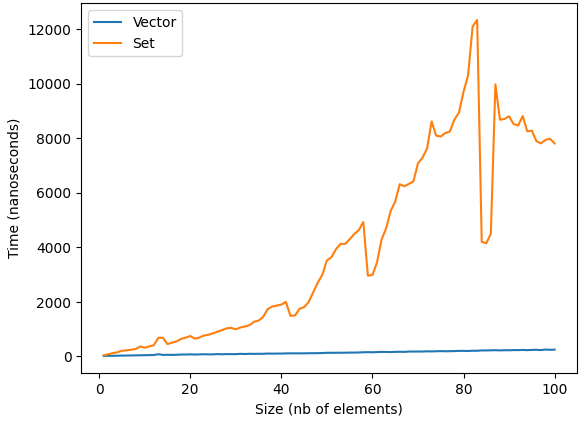
\includegraphics[width=9cm]{Diagram/insertion.png}
	\caption{Vector and set insertion times}
	\label{vector vs set insertion}
\end{figure}

We can see that when it comes to simple insertion, \code{vector} is significantly faster
than \code{unordered\_set}, at least for normal/small datasets.  This can be attributed to
the fact that optimized compilers often allocate memory in larger chunks when creating a
vector.  Since the dataset isn't very large, memory can be allocated only once for the
vector, unlike the unordered set. The variation in insertion time for the unordered set,
depending on the dataset size, can be explained by the occurrence of collisions. The
insertion time of an element in an unordered set depends on whether it creates a collision
or not.

\subsection{Look up}

Then we benchmarked the lookup, which means checking if a particular element is
contained. As mentioned earlier, for the vector, the entire container is tested one by one
until the value is found. This corresponds to linear complexity O(n). For the unordered
set, a simple hashing allows checking this information, which means constant complexity
O(1). We decided, in order to illustrate these different complexities well, to choose to
check if the container has its last element. The answer will always be yes, but
theoretically, it is the worst case scenario for the vector.

This is the exact benchmark procedure:
\begin{lstlisting}
	struct Test : Scenario<int> { Test(Container<int> *container) :
          Scenario<int>(container) {}
		
		void operator()(int data[], int length) override { container->lookup(target) } };
\end{lstlisting}


This algorithm will be executed much faster than the previous test.  To avoid measuring
noise, we took 1000 measurements per data set size with a step of 1. Here are the results
of the numerous measurements:
\begin{figure}[!h]
	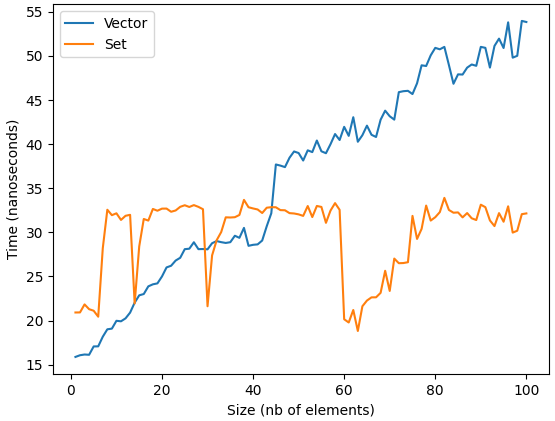
\includegraphics[width=9cm]{Diagram/lookup.png}
	\caption{Vector and set look up times}
	\label{vector vs set lookup}
\end{figure}

Despite our efforts, we can observe some instabilities in the curves, but the constant
nature of the unordered set and the linear nature of the vector are clearly visible, as
shown in the following diagram:
\begin{figure}[!h]
	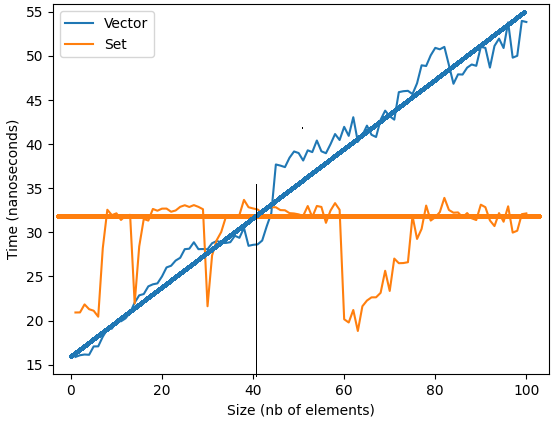
\includegraphics[width=9cm]{Diagram/lookup_courbe.png}
	\caption{Vector and set look up times simplified}
	\label{vector vs set lookup curve}
\end{figure}

We can see that initially, the lookup is faster for a vector than for an unordered set,
but from a data size of approximately 40, the vector becomes slower. Taking into account
the measurement uncertainties, we can estimate from these results that for a size below
30, the vector is faster for a lookup, for a size between 30 and 50, the difference is
negligible, and for a size above 50 elements, the unordered set is faster for a lookup. Of
course, this applies to our desktop environment on an x64 architecture and may not be
identical in all environments. For another environment, it would be preferable to re-run
the benchmark on it.

\section{Conclusion}

Our library allows for conducting small-scale benchmarks on various containers in the C++
language, including libraries such as STL. We were able to test its efficiency on the
example of \code{std::vector} vs \code{std::unordered\_set}. We were able to determine
from which data size it is faster to check if an element is present in a container for the
unordered set compared to the vector in our x64 environment. This information could assist
us in selecting the appropriate containers for our C++ programs, regardless of the
execution environment.

To ensure the quality of measurements through the benchmark, it is important to give high
priority to the benchmark process in the operating system and compile the program with
maximum optimizations.

Currently, the program only tests the \code{std::vector} and \code{std::unordered\_set}
containers, but it would be interesting to compare more containers, including other
libraries such as Boost.

\bibliographystyle{plain} \bibliography{ShortPaper-Refs.bib}

\end{document}
